\documentclass{article}
\usepackage[utf8]{inputenc}
\usepackage{comment}
\usepackage{biblatex}
\usepackage{multicol}
\addbibresource{references.bib}

\author{Eduardo Di Santi }
\date{June 2019}
\usepackage{graphicx}
\usepackage{comment}
\title{Solving Banana collector with deep reinforcement learning}
\begin{document}
\maketitle
\begin{abstract}
This document shows how to train a deep reinforcement learning agent with DQN to solve the Banana collector environment.
\end{abstract}

\section{Introduction}
The aim of the project is to train a Deep Reinforcement Learning agent to collect yellow bananas while avoiding blue bananas in a square world.

\begin{figure}[!htbp]
\centering
\includegraphics[scale=0.2]{bc1}
\caption{The environment}
\label{fig:bc1}
\end{figure}
This environment is a version of Unity ML-Agent Banana collector environment, suitable to test reinforcement algorithms. Solving this continuous spaces environment will need the use of an action value function approximation thru a deep neural network. 

\section{Environment}

The environment is a square world, the action state space has \textbf{37 dimensions} representing the agent speed and a ray-based\cite{ray-based} perception of objects around the agent forward direction.\newline
There reward is representing by an integer, \textbf{+1 (positive one)} for collecting a yellow banana and \textbf{-1 (negative one)} for collecting a blue banana.\newline
There is no reward, positive or negative for moving or time.\newline
The environment is considered solved when the agent can get a score of 13 over last 100 hundred consecutive episodes.\newline
The available actions are four as follows:
\begin{table}[!htbp]
\center
\begin{tabular}{l|l}
Action         & Value\\
\hline
Forward &     0   \\
Backward      & 1 \\
Left 	      & 2 \\
Right 	      & 3 	
\end{tabular}
\end{table}

\section{Algorithm}
The agent learns using a Deep Q-Learning \cite{dqn} algorithm with epsilon greedy exploration.\newline
This algorithm feed forwards a deep neural network with the state of the environment, after two hidden layers, the output layer activates is activated and the neuron with strongest signal is selected the fired one, meaning, the most probable best action is selected\newline.

The neural network used has the following architecture and hyper parameters
\begin{table}[!htbp]
\center
\begin{tabular}{1|1|1|1|1}
Layer         & Neurons   & Type & Activation & Comment  \\
\hline
Input  &  37 &	&	& according to the space state dimension\\
Hidden &  32 &	Linear &	ReLU \\	
Hidden &  32 &	Linear &	ReLU \\ 	
Output &   4 &	Linear &	ReLU & One for each action
\end{tabular}
\end{table}

The hyper parameters for the e-greedy exploration reinforcement learning are the following:
\begin{table}[!htbp]
\center
\begin{tabular}{l|l|l}
Parameter         & Value   & Description  \\
\hline
Replay start size &      0  & Replay memory initial size   \\
Replay size       & 100000  & Replay memory max size   \\
Batch size 	      &     32  & Batch size * Update every \\
Gamma 	          &   0.99 	& Discount rate \\
Hidden layers 	  & [32,32] & Q-Network \\
Tau 	          &    0.05 & Soft update rate \\
Update every 	  &      4 	& Learn every 4 \\
Learning rate 	  & 5e-05 	
\end{tabular}
\end{table}
\newline

\section{Results}
As expected, the agent learned how to play fast because the simplicity of the environment; when training, the agent showed a tendency to perform mostly the forward action, which is normal because is the action to get the banana, but, for correcting the direction, during the training the back action was performed more than half of the forward ones and at least twice more than left or right.
\subsection{When training}
The goal is to achieve an average score of 13 over last 100 episodes, with this hyper-parameters the agent solves the environment in 319 episodes.\newline
The agent achieve this score with following action - frequencies:
\begin{table}[!htbp] 
\center
\begin{tabular}{l|l|l}
Action         & Value & Frequency\\
\hline
Forward       & 0 & 57234 \\
Backward      & 1 & 25189 \\
Left 	      & 2 &  9690\\
Right 	      & 3 &	 4187
\end{tabular}
\end{table}
\newline The training history is as follows:
\begin{figure*}[ht!]
    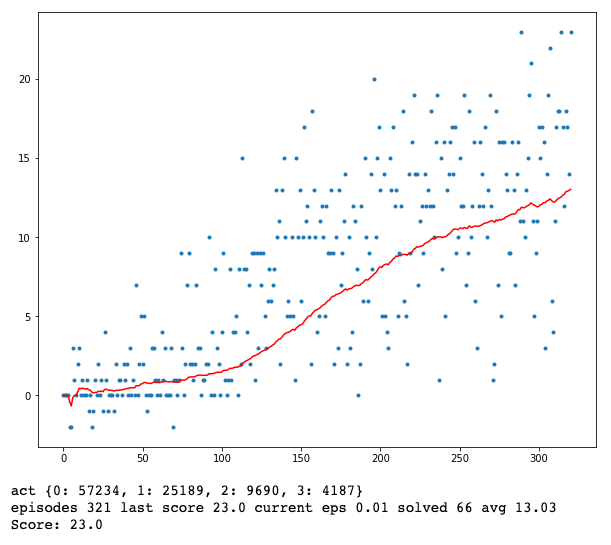
\includegraphics[scale=0.3]{training}\hfill
    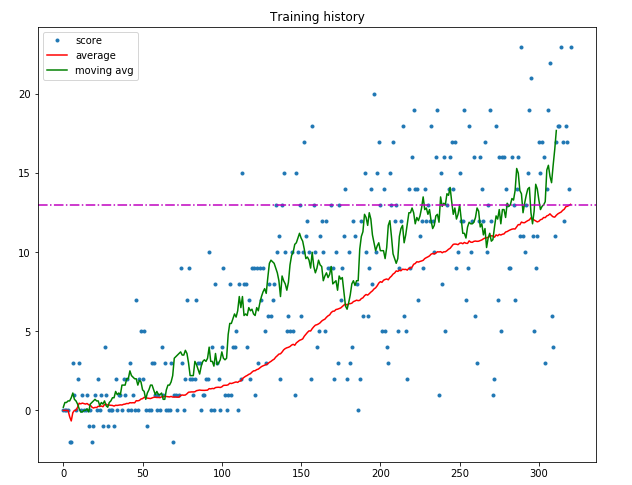
\includegraphics[scale=0.35]{training2}\hfill
    \caption{Training history, episodes vs rewards.}
    \caption{Training history, episodes vs rewards with moving average.}
\end{figure*}

\subsection{When playing}
Playing 100 trials with 2000 steps each, the agent performs as expected with little plays with some scores below 13:
\begin{figure}[!htbp]
\centering
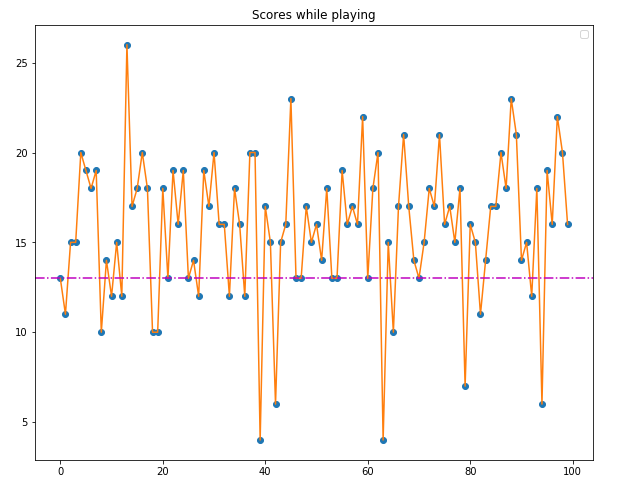
\includegraphics[scale=0.3]{play_scores}
\caption{Playing scores 100, episodes vs rewards}
\label{fig:play_scores}
\end{figure}

\section{Conclusions}
The agents performs very well solving the environment in the stated conditions, but its unable to solve the situation of being surrounded by blue bananas when yellow bananas are far away; the expected behaviour in this case, is to get a blue banana to go to a yellow bananas area.\newline
In those cases the agent just gives up by turning and moving searching for a hole in order to pass between blue bananas to avoid the negative rewards. Those cases has usually a return between 4 and 11.\newline
\section{Future work}
The DQN presents a high bias problem, so in future work changing the DQN by a prioritized experience play or a dueling DQN can improve the richness of actions learned.

\printbibliography
\end{document}
